\section{Runtime Layers and Continuity}
\label{sec:continuity-grammar}

The Elephant Agent layer model defines what persists, for how long, and under which
owner. The layers are ordered from durable understanding to atomic runtime
source material.

\begin{figure}[!t]
  \centering
  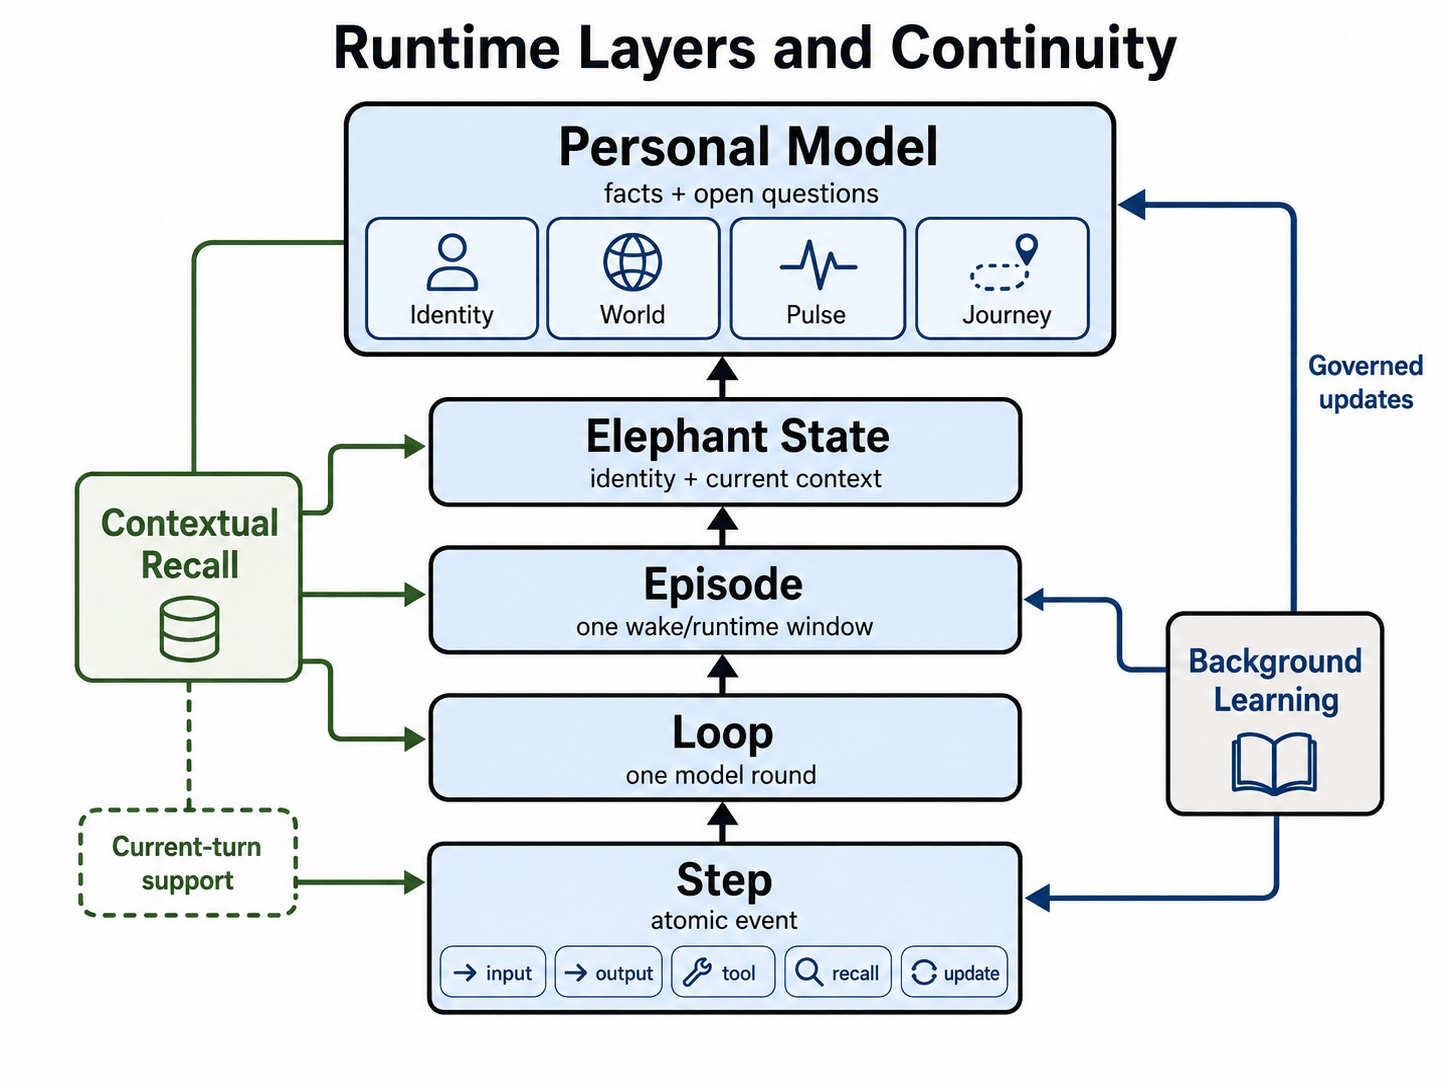
\includegraphics[width=0.86\linewidth]{../../apps/site/static/assets/resources/paper-6.png}
  \caption{The Elephant Agent system layer model, shown from atomic runtime material
  toward durable personalized understanding.}
  \label{fig:layer-model}
\end{figure}

\subsection{Step}

A Step is one atomic event inside a Loop. Examples include user input, model
response, tool call, tool result, recall, Personal Model update, or effective
user query. Steps are not durable memory owners. They are the finest-grained
source material for audit, replay, recovery, debugging, and later reflection.

This distinction prevents impressionistic personalization. Elephant Agent should not
learn directly from an opaque memory sentence. It should learn from structured
events whose source, order, outcome, and artifacts can be inspected.

\subsection{Loop}

A Loop is one model interaction round. It begins with a trigger and ends when
the model response, tool path, or handoff for that round is complete. A short
chat reply is a Loop. A long repair path with many tools may include multiple
Loops.

\subsection{Episode}

An Episode is one open runtime window: a wake, CLI shell window, gateway
worker, API handling window, or background runtime window. Ending an Episode
does not end continuity. A later wake opens a new Episode and resumes from the
same elephant State and Personal Model.

\subsection{Elephant State}

Elephant State is intentionally small:

\begin{center}
\texttt{elephant\_id, display\_name, identity\_text, current\_context\_note, updated\_at}
\end{center}

\texttt{current\_context\_note} is the State-level continuation note produced
by background Episode learning and copied into the next Episode's opening
resume snapshot. It is not a per-turn working memory field and must not become
a hidden task board. Live commitments belong in Episode, Step, current-turn
recall, or explicit task tools.

\subsection{Personal Model}

The Personal Model is the durable understanding layer. It is made of active,
retired, and disputed facts grouped by Identity, World, Pulse, and Journey, plus
open questions that may improve future help. It is not the elephant identity itself.
Deleting an elephant State does not imply deleting the Personal Model.

The simplifying rule is strict: only what should survive across multiple
States, Episodes, and surfaces belongs in the Personal Model. Everything else
should stay in Elephant State, Episode, Loop, Step, or current-turn recall.

\subsection{Wake and Resume}

Wake recovery combines Elephant State and Personal Model. Elephant Agent chooses the target
elephant, opens a new Episode, loads the State resume note, projects active Personal
Model facts, and may inject relevant \texttt{Current-turn recall support:} evidence for the
current turn.

The default wake packet should answer four product questions:

\begin{enumerate}[leftmargin=*]
  \item Who is this elephant and user relationship?
  \item Where did this continuity line leave off?
  \item Which active facts matter now?
  \item What evidence, if any, supports the current query?
\end{enumerate}

This packet is not the durable owner of continuity. It is a projection. If it
is wrong, the system should be able to show which facts, source Episodes, and
Steps produced it.
